\subsection{Decorators}
\label{sec:3_WC_Decorators}

Das folgende Kapitel basiert ausschließlich auf der Einführung zu Web-Components aus dem W3C \citereset \autocite[siehe][]{CooneyGlazkov.2013} und auf dem Artikel \glqq Decorators - NextGen Markup pt.2\grqq\ \citereset \autocite[siehe][]{PreventDefault.2013}.

Decorators sind Elemente, die nach dem Decorator-Pattern benannt sind. Zurzeit gibt es keinerlei Unterstützung seitens der Browser zu diesem Konzept, somit wird in dieser Arbeit das vom W3C definierte Konzept nur theoretisch erläutert. Um jedoch dieses Konzept vollständig verstehen zu können, wird zuerst das genannte Pattern kurz beschrieben.

Grundsätzlich gehört das Decorator-Pattern zu den Struktur-Pattern der Softwareentwicklung. Das Pattern dient als Alternative zu Vererbung. Unter der Annahme, dass ein Objekt einen Rahmen erhalten soll, kann dies mit zwei Konzepten gelöst werden: Einerseits durch Vererbung oder andererseits durch Komposition.

Bei Vererbung würde der Rahmen von einer anderen Klasse geerbt werden. Somit besitzen jedoch alle Sub-Klassen den Rahmen. Diese Methode ist sehr inflexibel, da der Rahmen statisch durch Vererbung erstellt wird. Eine Endbenutzerin beziehungsweise ein Endbenutzer hätte keine Kontrolle darüber, wie eine Komponente mit einem Rahmen versehen werden kann.

Ein flexibler Ansatz wäre, dass die Komponente von einem Objekt umgeben wird, dass einen Rahmen beinhaltet. Das umgebene Objekt wird auch \glqq Decorator\grqq\ genannt. Folgend wird dieser Ansatz an Hand von Abbildung \ref{fig:3_Decorator_UML} auf Seite \pageref{fig:3_Decorator_UML} näher beschrieben.

\begin{figure}[h]
\centering
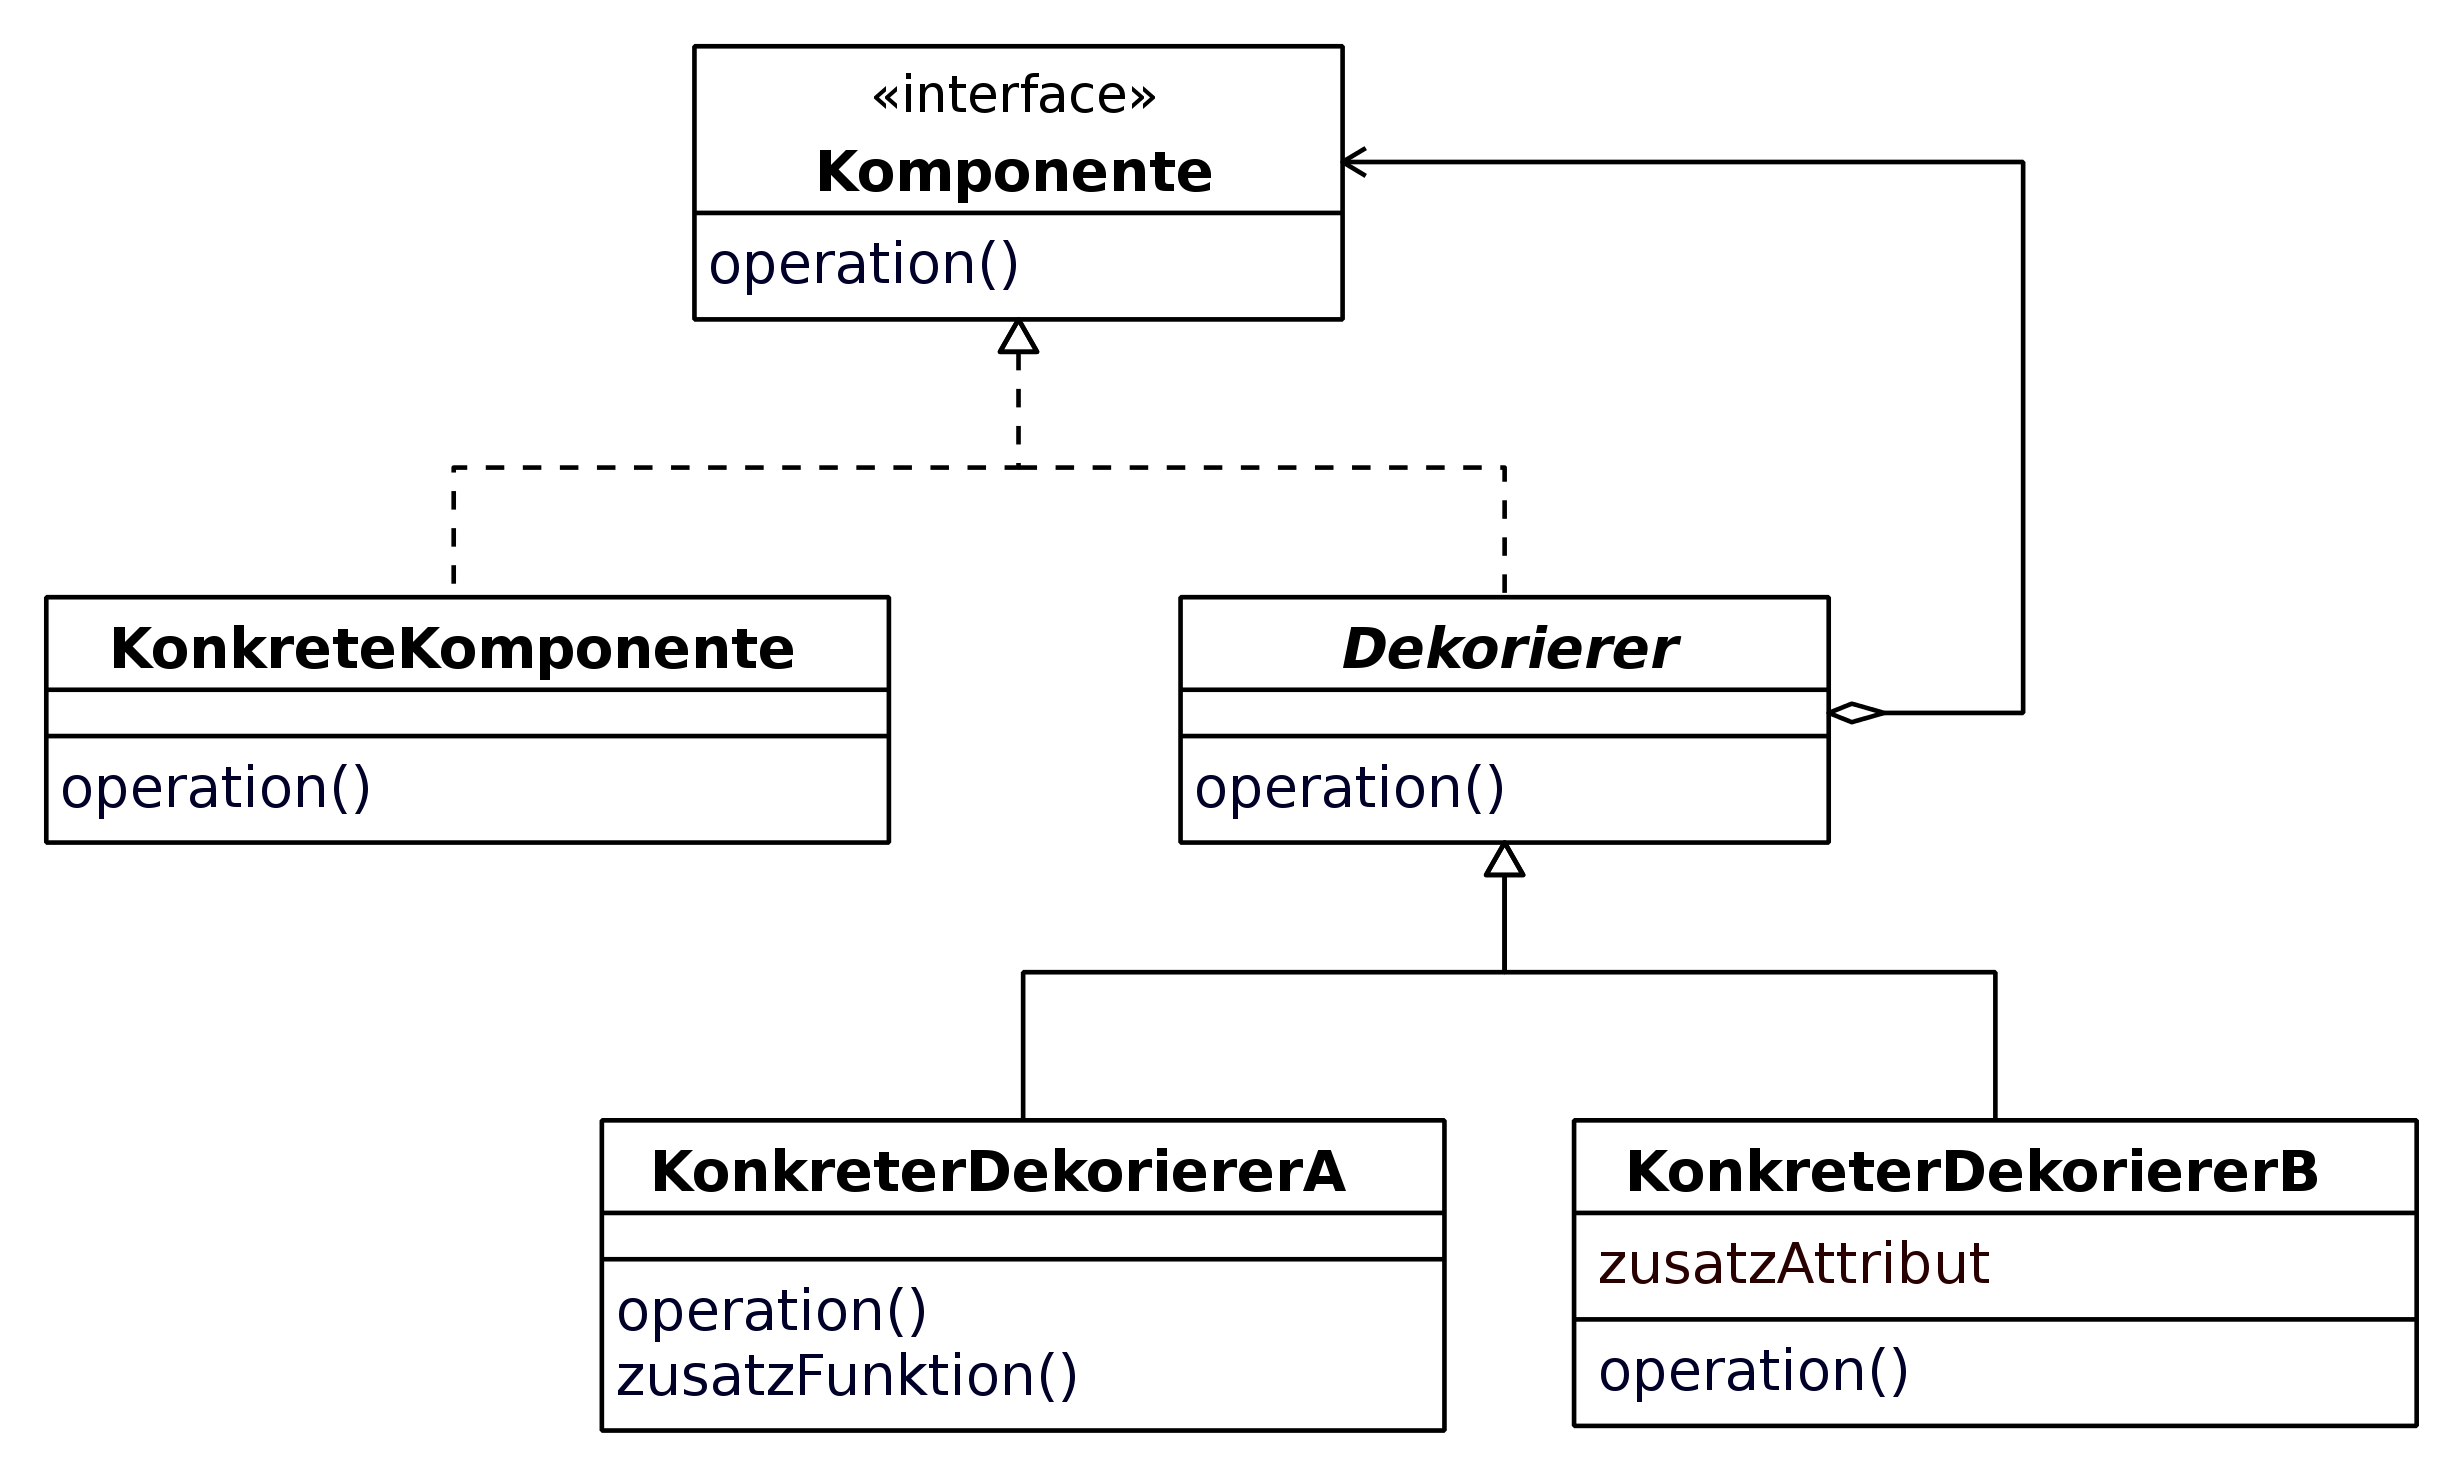
\includegraphics[height=5.0cm]{images/decorator.png}
\caption[
Decorator-Pattern UML
]{Decorator-Pattern UML \citereset \autocite[siehe][S. 196-200]{Gamma.1995}}
\label{fig:3_Decorator_UML}
\end{figure}

Der Decorator wird vor das zu dekorierende Objekt gelegt. Die abstrakte Komponente definiert öffentliche Schnittstellen für das zu dekorierende Objekt. Die konkrete Komponente definiert ein Objekt, das dekoriert werden kann. Der abstrakte Decorator beinhaltet eine Referenz auf eine konkrete Komponente und bietet dieselbe Schnittstelle wie die abstrakte Komponente an. Der konkrete Decorator definiert und implementiert eine oder mehrere spezielle Decorators.
Somit können Komponenten zur Laufzeit um zusätzliche Funktionalitäten und Darstellungen erweitern werden \citereset \autocite[siehe][S. 196-200]{Gamma.1995}.

Um Decorators mit Hilfe des W3C-Konzepts näher erklären zu können, wird in diesem Kapitel folgendes Beispiel verwendet. Es gibt eine Liste von Autos, wobei jedes Auto eine Modellbezeichnung, eine Marke, ein Bild, sowie eine Kurzbeschreibung hat. In Bezug auf das Decorator-Pattern (siehe Abbildung \ref{fig:3_Decorator_UML} auf Seite \pageref{fig:3_Decorator_UML}) wäre ein Auto eine konkrete Komponente. Das Markup eines Autos würde wie folgt aussehen:

\begin{lstlisting}[language=HTML, caption={[Web-Components Decorators - Markup eines Autos \citereset \autocite{PreventDefault.2013}] Web-Components Decorators - Markup eines Autos}, label={lst:3_Decorators_Basic}, escapeinside={@}{@}]
<li class="car-item">
   <img class="car-image" title="Seat Ibiza" src="images/seat-ibiza.jpg" />
   <h3 class="car-model">Seat Ibiza</h3>
   <p class="car-description">The SEAT Ibiza is a supermini car manufactured by the Spanish automaker SEAT. It is SEAT&#039;s best-selling car and perhaps the most popular model in the company&#039;s range.</p>
</li>
\end{lstlisting}

Folgend wird angenommen, dass die Funktionalität eines Autos erweitert wird: Ein Auto-Element bietet die Funktionalität, dass das Auto sichtbar, unsichtbar beziehungsweise geschlossen werden kann. Das bereits vorhandene Markup von Code-Beispiel \ref{lst:3_Decorators_Basic} auf Seite \pageref{lst:3_Decorators_Basic} wird somit wie folgt erweitert:

\begin{lstlisting}[language=HTML, caption={[Web-Components Decorators - Markup eines Autos mit Rahmen \citereset \autocite{PreventDefault.2013}] Web-Components Decorators - Markup eines Autos mit Rahmen}, label={lst:3_Decorators_Basic2}, escapeinside={@}{@}]
<li class="car-item">
   <section class="window-frame">
      <header>
          <a class="frame-toggle" href="#">Min/Max</a>
          <a class="frame-close" href="#">Close</a>
      </header>
      <img class="car-image" title="Seat Ibiza" src="images/seat-ibiza.jpg" />
      <h3 class="car-model">Seat Ibiza</h3>
      <p class="car-description">The SEAT Ibiza is a supermini car manufactured by the Spanish automaker SEAT. It is SEAT&#039;s best-selling car and perhaps the most popular model in the company&amp;#039;s range.</p>
   </section>
</li>
\end{lstlisting}

Code-Beispiel \ref{lst:3_Decorators_Basic2} auf Seite \pageref{lst:3_Decorators_Basic2} würde somit das Markup eines Autos und zwei Buttons beinhalten: einen zum Umschalten zwischen sichtbar und unsichtbar und einen um das Bild komplett zu schließen.
Wird das gezeigte Beispiel mit den bisherigen standardisierten Möglichkeiten umgesetzt, wird der Quellcode schnell relativ groß.

Decorators würden in diesem Beispiel bereits helfen. Es wäre möglich, spezielle Elemente im DOM mit mehr Markup, Gestaltung und zusätzlicher Funktionalität zu versehen. Essentiell hierbei ist, dass die zusätzliche Funktionalität nur für eine gewünschte Menge an Elementen erweitert werden kann. Hinsichtlich des bereits erklärten Decorator-Pattern wäre nachstehendes Code-Beispiel ein konkreter Decorator (siehe Abbildung \ref{fig:3_Decorator_UML} auf Seite \pageref{fig:3_Decorator_UML}). Die gewünschte Funktionserweiterung des Autos wird mit Hilfe eines Decorators umgesetzt. Das Markup würde somit wie folgt aussehen:

\begin{lstlisting}[language=HTML, caption={[Web-Components Decorators - Markup der zusätzlichen Funktionalität (Rahmen) \citereset \autocite{PreventDefault.2013}] Web-Components Decorators - Markup der zusätzlichen Funktionalität (Rahmen)}, label={lst:3_Decorators_Basic3}, escapeinside={@}{@}]
<decorator id="frame-decorator">
   <template>
      <section id="window-frame">
         <header>
            <a id="toggle" href="#">Min/Max</a>
            <a id="close" href="#">Close</a>
         </header>
         @\label{lst:3_Decorators_Basic3_content}@<content></content>
      </section>
   </template>
</decorator>
\end{lstlisting}

Decorators werden grundsätzlich mit \lstinline|<template>|-Elementen eingesetzt (mehr zu Templates in Kapitel \ref{sec:3_WC_Templates} auf Seite \pageref{sec:3_WC_Templates}). Des Weiteren wird in Zeile \ref{lst:3_Decorators_Basic3_content} des Code-Beispiels \ref{lst:3_Decorators_Basic3} ein \lstinline|<content>|-Element verwendet. Dies ist zwingend notwendig, da in dieser Stelle der Inhalt des zu dekorierenden Elements eingefügt wird. In diesem \lstinline|<content>|-Element wird somit die Referenz der Komponente, die der Decorator beinhaltet, eingefügt.
Auch ist zu erwähnen, dass in diesem Beispiel nur \lstinline|IDs| verwendet werden. Dies dient der Visualisierung, dass \lstinline|IDs| innerhalb eines \lstinline|<decorator>|-Elements gekapselt sind. Sie werden nie im DOM erscheinen beziehungsweise verfügbar sein. \lstinline|document.getElementById("window-frame")| wird keine Elemente zurückgeben, weder vor noch nach der Anwendung des \lstinline|<decorator>|-Elements.

Weiterhin ist es möglich, sämtliche Elemente eines Decorators zu gestalten. In Code-Beispiel \ref{lst:3_Decorators_Basic4} auf Seite \pageref{lst:3_Decorators_Basic4} werden die beiden Buttons mit \lstinline|float: right;| gestaltet. Um die \lstinline|floats| der Elemente wieder zu löschen, wird das \lstinline|<header>|-Element mit der CSS-Klasse \lstinline|clearfix| erweitert.

\begin{lstlisting}[language=HTML, caption={[Web-Components Decorators - Markup der zusätzlichen Funktionalität (Rahmen) inklusive Style \citereset \autocite{PreventDefault.2013}] Web-Components Decorators - Markup der zusätzlichen Funktionalität (Rahmen) inklusive Style}, label={lst:3_Decorators_Basic4}, escapeinside={@}{@}, escapechar=!]
<decorator id="frame-decorator">
   <template>
      <section id="window-frame">
        !\colorbox{light-gray}{<style scoped>}!
            !\colorbox{light-gray}{\#toggle {float: right;}}!
            !\colorbox{light-gray}{\#close {float: right;}}!
         !\colorbox{light-gray}{</style>}!
         !\colorbox{light-gray}{<header class="clearfix">}!
            <a id="toggle" href="#">Min/Max</a>
            <a id="close" href="#">Close</a>
         </header>
         <content></content>
      </section>
   </template>
</decorator>
\end{lstlisting}

Es ist zu beachten, dass sämtliche Gestaltungen außerhalb des \lstinline|<style scoped>|-Elements unter Verwendung der richtigen Klassennamen immer noch angewendet werden.

Um nun das bereits vorhandene Markup mit Funktionalität versehen zu können, muss zuerst noch ein wichtiger Punkt bezüglich Events erläutert werden. Bei Decorators gibt es keine \glqq normalen\grqq\ Events. Das Hinzufügen beziehungsweise Entfernen eines Decorators würde das Event, wenn es bereits auf ein Element gebunden war, löschen. Decorators bieten nun die Möglichkeit einen Event-Controller zu erstellen, um mit Hilfe von diesen Events verwalten zu können.

\begin{lstlisting}[language=HTML, caption={[Web-Components Decorators - Markup der zusätzlichen Funktionalität (Rahmen) inklusive Style und Funktionalität \citereset \autocite{PreventDefault.2013}] Web-Components Decorators - Markup der zusätzlichen Funktionalität (Rahmen) inklusive Style und Funktionalität}, label={lst:3_Decorators_Basic5}, escapeinside={@}{@}, escapechar=!]
<decorator id="frame-decorator">
   <script>
      this.listen({
         selector:"#toggle", type:"click",
         handler: function (event) {
            // do the toggle button logic here
         }
      });
      this.listen({
         selector:"#close", type:"click",
         handler: function (event) {
            // do the close button logic here
         }
      });
   </script>
   <template>
      <section id="window-frame">
         <style scoped>
            #toggle {float: right;}
            #close {float: right;}
         </style>
         <header class="clearfix">
            <a id="toggle" href="#">Min/Max</a>
            <a id="close" href="#">Close</a>
         </header>
         <content></content>
      </section>
   </template>
</decorator>
\end{lstlisting}

Der in Code-Beispiel \ref{lst:3_Decorators_Basic5} auf Seite \ref{lst:3_Decorators_Basic5} gezeigte Decorator kann somit verwendet werden, um die gewünschte Funktionalität (das Bild des Autos soll sichtbar, unsichtbar beziehungsweise geschlossen werden können) bereitstellen zu können, ohne dabei für jedes \lstinline|<li>|-Element extra Markup hinzufügen zu müssen. Schlussendlich würde das Beispiel für ein Auto wie folgt aussehen:

\begin{lstlisting}[language=HTML, caption={[Web-Components Decorators - Markup eines Autos mit Decorator \citereset \autocite{PreventDefault.2013}] Web-Components Decorators - Markup eines Autos mit Decorator}, label={lst:3_Decorators_Basic6}, escapeinside={@}{@}, escapechar=!]
<decorator id="frame-decorator">
   <script>
      this.listen({
         selector:"#toggle", type:"click",
         handler: function (event) {
            // do the toggle button logic here
         }
      });
      this.listen({
         selector:"#close", type:"click",
         handler: function (event) {
            // do the close button logic here
         }
      });
   </script>
   <template>
      <section id="window-frame">
         <style scoped>
            #toggle {float: right;}
            #close {float: right;}
         </style>
         <header class="clearfix">
            <a id="toggle" href="#">Min/Max</a>
            <a id="close" href="#">Close</a>
         </header>
         <content></content>
      </section>
   </template>
</decorator>

<li class="car-item">
   <img class="car-image" title="Seat Ibiza" src="images/seat-ibiza.jpg" />
   <h3 class="car-model">Seat Ibiza</h3>
   <p class="car-description">The SEAT Ibiza is a supermini car manufactured by the Spanish automaker SEAT. It is SEAT&#039;s best-selling car and perhaps the most popular model in the company&#039;s range.</p>
</li>
\end{lstlisting}

\begin{lstlisting}[language=CSS, caption={[Web-Components Decorators - CSS für die Verwendung von Decorators \citereset \autocite{PreventDefault.2013}] Web-Components Decorators - CSS für die Verwendung von Decorators}, label={lst:3_Decorators_Basic7}, escapeinside={@}{@}, escapechar=!]
.car-item {
  decorator: url(#frame-decorator);
}
\end{lstlisting}

Unter der Verwendung des in Code-Beispiel \ref{lst:3_Decorators_Basic7} auf Seite \pageref{lst:3_Decorators_Basic7} gezeigten CSS-Attributs wird der Decorator für das in Code-Beispiel \ref{lst:3_Decorators_Basic6} auf Seite \pageref{lst:3_Decorators_Basic6} gezeigte Markup verwendet. Mit Hilfe des \lstinline|decorator:| Attribut in CSS kann die URL beziehungsweise die Id des definierten Decorators angegeben werden. Das HTML-Element, das die CSS-Klasse mit dem gegebenen \lstinline|decorator|-Attribut besitzt, wird mit dem im \lstinline|<decorator id='frame-decorator'>| definierten Markup versehen. In Bezug zu dem Decorator-Pattern wäre dies der Vorgang, wo der Decorator vor die Komponente, sprich in unserem Fall vor ein Auto, gesetzt wird. Weiters kann dieser Decorator vor spezielle Elemente gesetzt werden. Somit müssen nicht alle Autos die Funktionserweiterung erhalten.
